\documentclass[a4paper, 12pt]{article}
\usepackage[a4paper,top=1.5cm, bottom=1.5cm, left=1cm, right=1cm]{geometry}
\usepackage{cmap}					% поиск в PDF
\usepackage{mathtext} 				% русские буквы в формулах
\usepackage[T2A]{fontenc}			% кодировка
\usepackage[utf8]{inputenc}			% кодировка исходного текста
\usepackage[english,russian]{babel}	% локализация и переносы

\usepackage{amsmath}
\usepackage{indentfirst}
\usepackage{longtable}
\usepackage{graphicx}
\usepackage{array}

\usepackage{wrapfig}
\usepackage{siunitx} % Required for alignment
\usepackage{subfigure}
\usepackage{multirow}
\usepackage{rotating}
\usepackage{caption}

\graphicspath{{.}}


\title{\begin{center}Лабораторная работа №2.5.1\end{center}
Измерение коэффициента поверхностного натяжения жидкости}
\author{Рожков А. В. \\ Преподаватель Яворский В. А.}
\date{\today}

\begin{document}
    \pagenumbering{gobble}
    \maketitle
    \newpage
    \pagenumbering{arabic}

    \textbf{Цель работы:} 1) измерение температурной зависимости коэффициента поверхностного натяжения дистиллированной воды с использованием известного коэффициента поверхностного натяжения спирта; 2) определение полной поверхностной энергии и теплоты, необходимой для изотермического образования единицы поверхности жидкости при различной температуре.

	\textbf{В работе используются:} прибор  Ребиндера  с термостатом ($\sigma_T = 0.1~^oC$) и микроманометром ($k = 0.2$; $\rho_{ман} = 785.3~кг/м^3$; $\sigma_h = 1~мм$); исследуемые жидкости; стаканы; микроскоп ($\sigma_d = 0.05~мм$).

    \section{Теоретические сведения}

	Наличие поверхностного слоя приводит к различию давлений по разные стороны от искривленной границы раздела двух сред.  Для сферического пузырька с воздухом  внутри жидкости избыточное давление дается формулой Лапласа:

	\begin{equation}
		\Delta P = P_{int} - P_{ext} = \frac{2\sigma}{r},
		\label{key}
	\end{equation}
	где $ \sigma $ -- коэффициент поверхностного натяжения, $ P_{int} $ и $ P_{ext} $ -- давление внутри пузырька и снаружи, $ r $ -- радиус кривизны поверхности раздела двух фаз. Эта формула лежит в основе предлагаемого метода определения коэффициента поверхностного натяжения жидкости. Измеряется давление $ \Delta P $, необходимое для выталкивания в жидкость пузырька воздуха.

	\section{Экспериментальная установка}

    \begin{figure}[!ht]
        \begin{center}
            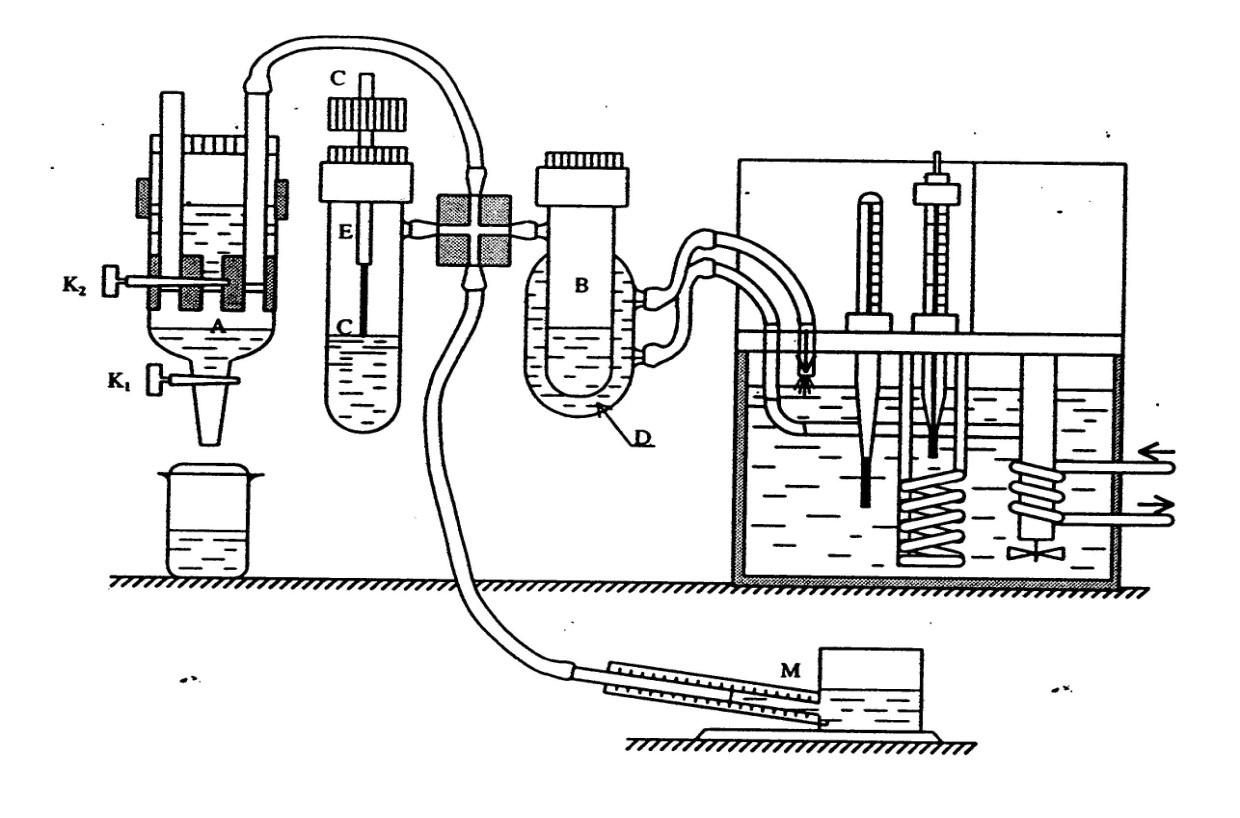
\includegraphics[width=0.6 \textwidth]{img/ust.jpg}
        \end{center}
        \caption{Экспериментальная установка}
		\label{img:ust}
    \end{figure}

	Исследуемая жидкость (дистиллированная вода) наливается в сосуд (колбу) $ B $ (рис. \eqref{img:ust}). Тестовая жидкость  (этиловый спирт) наливается  в сосуд $ E $.  При измерениях  колбы герметично закрываются  пробками. Через одну из двух пробок  проходит полая металлическая игла $ С $. Этой пробкой закрывается сосуд, в котором  проводятся измерения. Верхний конец иглы открыт в атмосферу, а нижний погружен в жидкость. Другой сосуд герметично закрывается второй пробкой. При создании достаточного  разряжения воздуха в колбе с иглой пузырьки воздуха начинают пробулькивать через жидкость. Поверхностное натяжение можно определить по величине разряжения $ \Delta P $ \eqref{key}, необходимого для прохождения пузырьков (при известном радиусе иглы).

	Разряжение в системе создается с помощью аспиратора $ A $. Кран $ K_2 $ разделяет две полости аспиратора. Верхняя полость при закрытом кране $ K_2 $ заполняется водой. Затем кран $ K_2 $ открывают и заполняют водой  нижнюю полость  аспиратора.  Разряжение воздуха создается в нижней полости  при открывании крана $ K_1 $, когда  вода вытекает из неё по каплям. В колбах $ В $ и $ С $, соединённых трубками с нижней полостью аспиратора, создается такое же пониженное давление. Разность давлений в полостях с разряженным воздухом и атмосферой измеряется спиртовым микроманометром.

	Для стабилизации температуры исследуемой жидкости через рубашку $ D $ колбы $ В $ непрерывно прогоняется вода из термостата.

	Обычно кончик иглы лишь касается поверхности жидкости, чтобы исключить влияние гидростатического давления столба жидкости. Однако при измерении температурной зависимости коэффициента поверхностного натяжения возникает ряд сложностей. Во-первых, большая теплопроводность металлической трубки приводит к тому, что температура на конце трубки заметно ниже, чем в глубине жидкости. Во-вторых, тепловое расширение поднимает уровень жидкости при увеличении температуры.

	Обе погрешности можно устранить, погрузив кончик трубки до самого дна. Полное давление, измеренное при этом микроманометром, равно \[ P = \Delta P + \rho g h.\] Заметим, что $ \rho gh $ от температуры практически не зависит, так как подъём уровня жидкости компенсируется уменьшением её плотности (произведение $ \rho g $ определяется массой всей жидкости и поэтому постоянно). Величину  $ \rho g h $ следует измерить двумя способами.

	Во-первых, замерить величину $ P_1= \Delta P' $, когда кончик трубки только касается поверхности жидкости. Затем при этой же температуре опустить иглу до дна и замерить $ P_2= \rho gh + \Delta P'' $ ($ \Delta P' $, $ \Delta P'' $ -- давление Лапласа). Из-за  несжимаемости  жидкости можно положить $ \Delta P' = \Delta P'' $ и тогда \[ \rho gh= P_2 - P_1. \]

	Во-вторых, при измерениях $ P_1 $ и $ P_2 $ замерить линейкой  глубину погружения иглы $ h $. Это можно сделать, замеряя расстояние между верхним концом иглы и любой неподвижной частью прибора при положении иглы на поверхности и в глубине колбы.

	\section{Ход работы}

		\subsection{Проверка герметичности установки}

			Для проверки опускаем чистую сухую иглу в сосуд со спиртом так, чтобы кончик иглы лишь касался поверхности спирта. Плотно закрываем обе колбы и открываем кран аспиратора для пробулькивания пузырьков воздуха в колбе. Замеряем показания микроманометра, они не должны меняться.

		\subsection{Начало измерений}

			Положением крана аспиратора подбираем частоту падения капель так, чтобы максимальное давление манометра не зависело от этой частоты (не чаще чем 1 капля в 5 секунд).

		\subsection{Определение диаметра иглы}
			\label{needle_diam}

			Параметры при измерениях:

			\begin{align*}
				t_{комн} &= 25~^oC & \sigma_{спирт} &= 22.3~\frac{мН}{м}
			\end{align*}

			Измеряем максимальное давление $\Delta P_{спирт}$ при пробулькивании пузырьков воздуха через спирт.

			Провели 10 измерений. Показания манометра для всех $h_{ман} = 43~мм$. Значит случайная погрешность измерений равна 0. Результат с приборной погрешностью:

			\begin{align*}
				\Delta P_{спирт} &= \rho_{ман} g h_{ман} k = (66 \pm 2)~Па \\
				d &= \frac{4 \sigma_{спирт}}{\Delta P_{спирт}} = (1.35 \pm 0.04)~мм
			\end{align*}

			Измеряем диаметр внутреннего отверстия иглы при помощи микроскопа в двух направлениях:

			\begin{figure*}[ht!]
				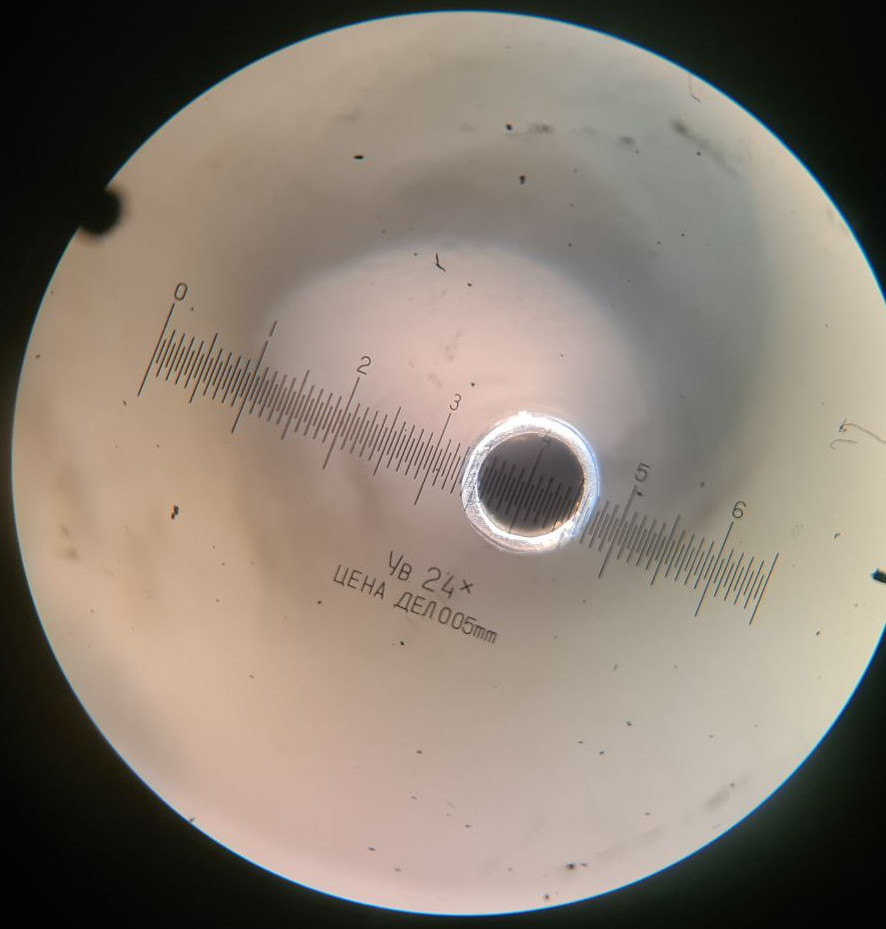
\includegraphics[width=.49\textwidth]{img/microscope1}\hfill
				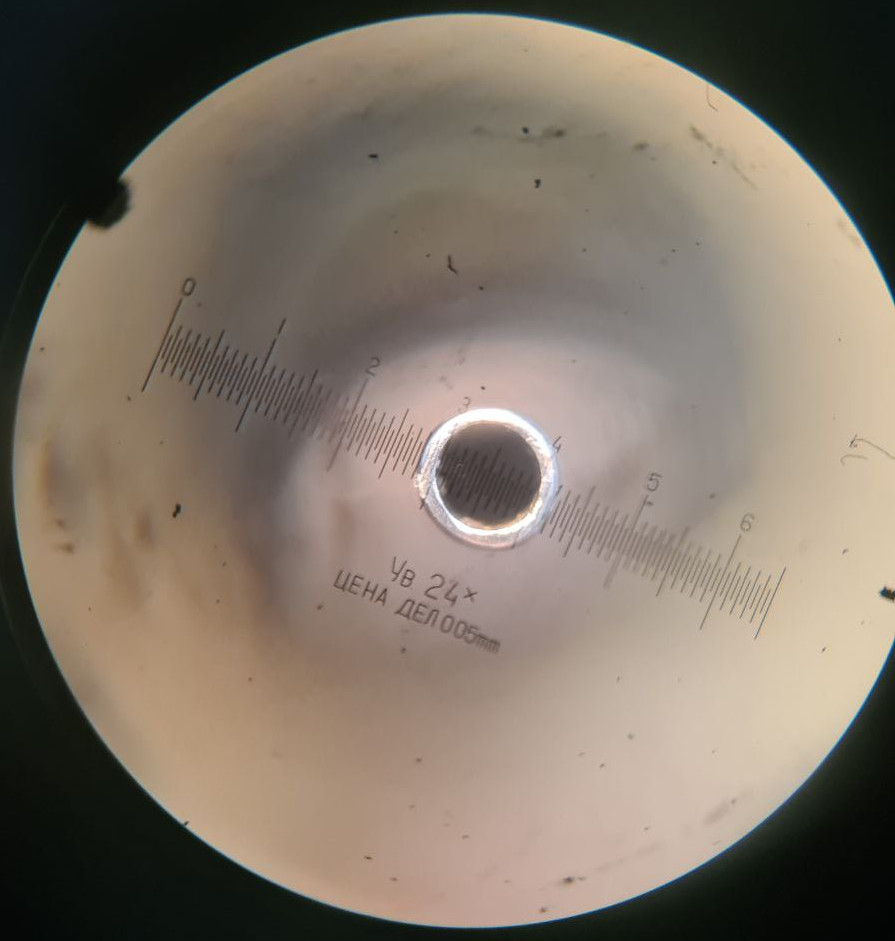
\includegraphics[width=.49\textwidth]{img/microscope2}
				\caption{Измерение диаметра иглы микроскопом}
			\end{figure*}

			\begin{align*}
				d_1 &= (1.10 \pm 0.05)~мм & d_2 &= (1.05 \pm 0.05)~мм \\
				sigma_d &= \sqrt{\sigma_d^{приб^2} + \sigma_d^{случ^2}} = \sqrt{\sigma_d^{приб^2} + \frac{1}{2}\sum_{i=1}^2(d_i - \langle d \rangle)^2} \\
				d_{игла} &= \frac{d_1 + d_2}{2} = (1.08 \pm 0.06)~мм
			\end{align*}

			Результат, измеренный микроскопом меньше экспериментального значения на $0.27~мм$. Такое расхождение можно объяснить несколькими причинами:
			\begin{itemize}
				\item температура иглы не совпадает с температурой спирта (в дальнейшем эту причину исключим, погрузив иглу в спирт);
				\item во время эксперимента за короткий промежуток времени из иглы пробулькивало сразу по 2 пузырька воздуха;
				\item игла может быть загрязнена жиром (или другими ПАВ).
			\end{itemize}

			Далее будем использовать диаметр иглы, измеренный микроскопом, как более точный.

		\subsection{Измерения для дистиллированной воды с иглой на поверхности}

			Промываем и просушиваем иглу. Далее приводим её в соприкосновение с поверхностью дистиллированной воды. Регулируем скорость поднятия уровня спирта в манометре и измеряем максимальное давление пробулькивания пузырьков $P_1$. Также измеряем расстояние между верхним концом иглы и неподвижным торцом сосуда $h_2$.

			\begin{align*}
				P_1 &= (182 \pm 2)~Па\\
				h_1 &= (21.5 \pm 0.5)~мм
			\end{align*}

			\subsubsection{Определение коэффициента поверхностного натяжения воды по известном значению для спирта}

				Зная коэффициент поверхностного натяжения спирта $\sigma_{спирт} = 22.3~\frac{мН}{м}$ при комнатной температуре ($25^oC$), можно найти соответствующий коэффициент для воды по формуле:

				\begin{align*}
					\sigma_{вода} &= \sigma_{спирт} \frac{h_{вода}}{h_{спирт}} = 22.3~\frac{мН}{м} * \frac{118~мм}{43~мм} = 61~\frac{мН}{м}\\
					\sigma_{\sigma_{вода}} &= \sigma_{вода} \sqrt{\left( \frac{\sigma_{\sigma_{спирт}}}{\sigma_{спирт}} \right)^2 + \left( \frac{\sigma_{h_{вода}}}{h_{вода}} \right)^2 + \left( \frac{\sigma_{h_{спирт}}}{h_{спирт}} \right)^2} = 2~\frac{мН}{м}
				\end{align*}

				Такой метод измерений нельзя назвать точным, так как табличное значение равно $71.99~\frac{мН}{м}$. Расхождение можно объяснить теми же причинами, что и в предыдущем пункте.

		\subsection{Измерения для дистиллированной воды с погружённой иглой}

			Опускаем иглу максимально вниз в воду. Измеряем расстояние $h_2$ как в предыдущем пункте. Измеряем максимальное давление $P_2$.

			\begin{align*}
				P_2 &= (289 \pm 3)~Па\\
				h_2 &= (6.5 \pm 0.5)~мм
			\end{align*}

			По разности давлений $\Delta P = P_2 - P_1$ определим глубину погружения $\Delta h$ иглы и сравним с $\Delta h = h_1 - h_2$. Плотность воды при комнатной температуре ($25^oC$) $\rho_{вода} = 997.0~кг/м^3$

			\begin{align*}
				\Delta P &= P_2 - P_1 = (108 \pm 4)~Па\\
				\Delta h &= \frac{\Delta P}{\rho_{вода} g} = (11.0 \pm 0.4)~мм\\
				\Delta h &= h_1 - h_2 = (15.0 \pm 0.7)~мм
			\end{align*}

			Значения $\Delta h$ отличаются на $4~мм$. Это можно объяснить теми же причинами, что и в пункте \ref{needle_diam}.

		\subsection{Температурная зависимость $\sigma(T)$}

			Включаем термостат и дожидаемся установления температуры около $25^oC$ в течение 5 минут. Проводим 5 измерений максимального давления. Далее то же для всех исследуемых температур.

			\begin{align*}
				P &= \rho_{ман} g h_{ман} k \\
				\sigma_P &= P \sqrt{\left( \frac{\sigma_{\rho_{ман}}}{\rho_{ман}} \right)^2 + \left( \frac{\sigma_g}{g} \right)^2 + \left( \frac{\sigma_h}{h} \right)^2}
			\end{align*}

			Во всех группах по 5 измерений показания манометра оставались стабильными, значит случайная погрешность измерений равна 0. Результаты измерений в таблице \ref{tab:sigma_T}.

		\subsection{Расчёт величины коэффициента поверхностного натяжения}

			Используя полученные в эксперименте показания манометра, а также измеренный микроскопом диаметр иглы, найдём величину коэффициента поверхностного натяжения для каждой температуры. Из уравнения (\ref{key}):

			\begin{align*}
				\sigma &= \frac{d_{игла} P}{4}\\
				\sigma_{\sigma} &= \sigma \sqrt{ \left( \frac{\sigma_{d_{игла}}}{d_{игла}} \right)^2 + \left( \frac{\sigma_P}{P} \right)^2}
			\end{align*}

			Результаты в таблице \ref{tab:sigma_T}.

			\begin{table}[!ht]
				\centering
				\begin{tabular}{|c|c|c|c|c|}
					\hline

					№ & $T, K$ & $h, мм$ & $P, Па$ & $\sigma, мН/м$\\ \hline
					1 & $298.3 \pm 0.1$ & $188 \pm 1$ & $289 \pm 3$ & $78 \pm 4$\\ \hline
					2 & $300.4 \pm 0.1$ & $187 \pm 1$ & $288 \pm 3$ & $77 \pm 4$\\ \hline
					3 & $303.4 \pm 0.1$ & $186 \pm 1$ & $286 \pm 3$ & $77 \pm 4$\\ \hline
					4 & $306.4 \pm 0.1$ & $185 \pm 1$ & $285 \pm 3$ & $77 \pm 4$\\ \hline
					5 & $309.3 \pm 0.1$ & $184 \pm 1$ & $283 \pm 3$ & $76 \pm 4$\\ \hline
					6 & $312.3 \pm 0.1$ & $184 \pm 1$ & $283 \pm 3$ & $76 \pm 4$\\ \hline
					7 & $315.2 \pm 0.1$ & $183 \pm 1$ & $282 \pm 3$ & $76 \pm 4$\\ \hline
					8 & $318.2 \pm 0.1$ & $182 \pm 1$ & $280 \pm 3$ & $75 \pm 4$\\ \hline
					9 & $321.3 \pm 0.1$ & $181 \pm 1$ & $279 \pm 3$ & $75 \pm 4$\\ \hline

				\end{tabular}
				\caption{Результаты измерений зависимости $\sigma(T)$}
				\label{tab:sigma_T}
			\end{table}

		\subsection{График зависимости $\sigma(T)$}

			\begin{figure}[!ht]
				\centering
				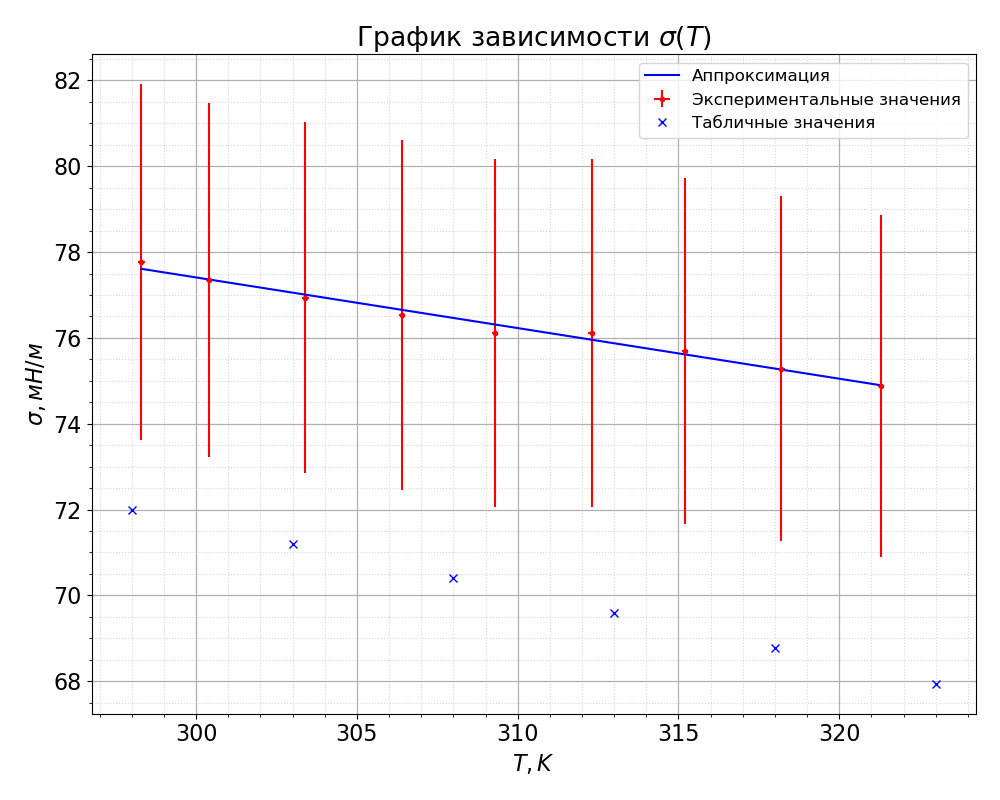
\includegraphics[width=0.75\textwidth]{graph/sigma_T_plot.png}
				\caption{График зависимости $\sigma(T)$}
				\label{plot:dsigma_div_dT}
			\end{figure}

			По коэффициенту наклона графика \ref{plot:dsigma_div_dT} определяем $\frac{d\sigma}{dT}$:

			\begin{align*}
				\sigma_{\frac{d\sigma}{dT}} &= \sqrt{k^2 \left( \left( \frac{\sigma_{d_{игла}}}{d_{игла}} \right)^2 + \left( \frac{\sigma_P}{P} \right)^2 + \left( \frac{\sigma_T}{T} \right)^2 \right) + \sigma_k^{случ^2}}\\
				\frac{d\sigma}{dT} &= (-118 \pm 9)~\frac{мкН}{м*К}
			\end{align*}

			Из закона Кирхгофа $\frac{С_{P(П)} - C_{P(Ж)}}{L_0} = \frac{\left( \frac{d\sigma}{dT} \right)}{\sigma_0} $, где $С_{P(П)} = 34~\frac{Дж}{моль*К}$ -- молярная теплоёмкость водяного пара при постоянном давлении; $С_{P(Ж)} = 76~\frac{Дж}{моль*К}$ -- молярная теплоёмкость воды; $L_0 = 44~\frac{кДж}{моль}$ -- молярная теплота парообразования воды при комнатной температуре $25^oC$; $\sigma_0 = (78 \pm 4)~\frac{мН}{м}$ -- коэффициент поверхностного натяжения дистиллированной воды при комнатной температуре $25^oC$.

			Из вышеприведённого соотношения имеем уравнение (\ref{eq:kirhgoff}). Рассчитаем левую часть и сравним с правой.

			\begin{equation}
				\frac{С_{P(П)} - C_{P(Ж)}}{L_0} \sigma_0 = \left( \frac{d\sigma}{dT} \right)
				\label{eq:kirhgoff}
			\end{equation}

			\begin{align*}
				\frac{С_{P(П)} - C_{P(Ж)}}{L_0} \sigma_0 &= (-74 \pm 4)~\frac{мкН}{м*К}\\
				\left( \frac{d\sigma}{dT} \right) &= (-118 \pm 9)~\frac{мкН}{м*К}
			\end{align*}

			Табличное значение $\frac{d\sigma}{dT} = -133~\frac{мкН}{м*К}$

			Расхождения в значениях опять же можно объяснить загрязнённостью иглы или дистиллированной воды. На иглу могли попасть поверхностно-активные вещества (ПАВ), которые увеличили коэффициент поверхностного натяжения. Именно это мы видим на графике \ref{plot:dsigma_div_dT}.

		\subsection{Графики зависимости $q(T)$ и $\frac{U}{F}(T)$}

			Построим графики зависимости от температуры:

			\begin{enumerate}
				\item теплоты образования единицы поверхности жидкости: $q = - T \frac{d \sigma}{dT}$ и
				\item поверхностной энергии $U$ единицы площади $F$: $\frac{U}{F} = \left( \sigma - T \frac{d \sigma}{dT} \right)$.
			\end{enumerate}

			\begin{figure}[!ht]
				\centering
				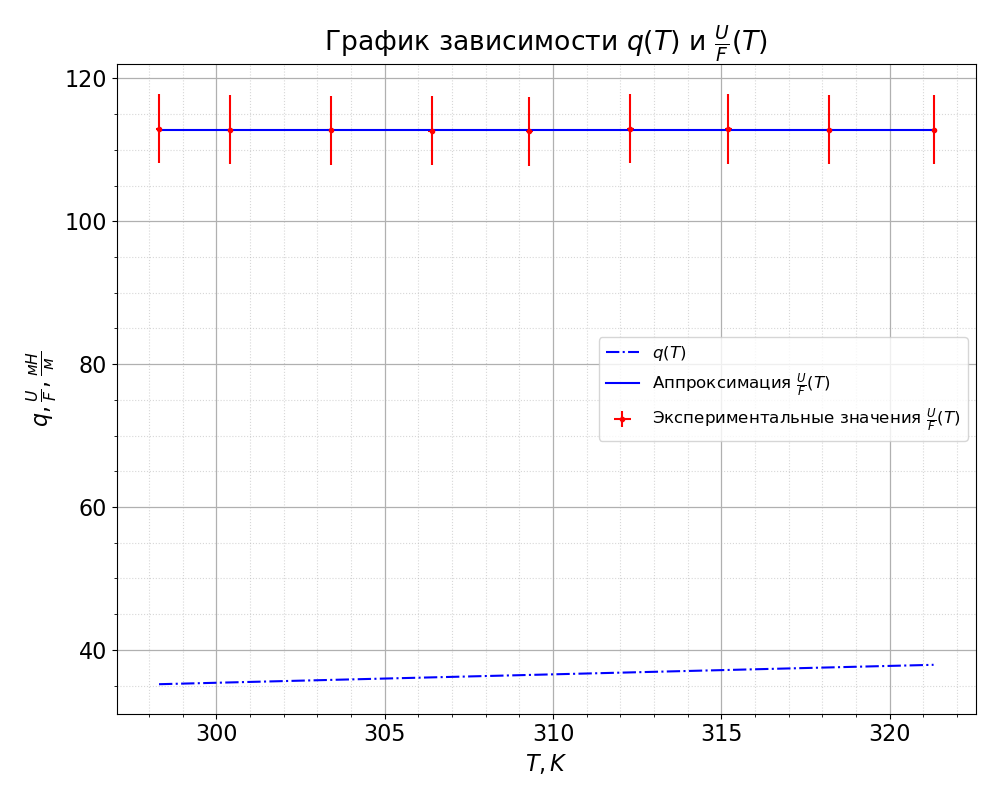
\includegraphics[width=0.75\textwidth]{graph/q_T_and_U_div_F_T_plot.png}
				\caption{График зависимости $q(T)$ и $\frac{U}{F}(T)$}
				\label{plot:q_and_U_div_F}
			\end{figure}

			Заметим, что процесс действительно изотермический, так как прямая $\frac{U}{F}(T)$ почти горизонтальная ($k = 1.05$).

	\section{Вывод}

		В ходе работы измерили температурную зависимость коэффициента поверхностного натяжения дистиллированной воды при различной температуре. А также определили полную поверхностную энергию и теплоту, необходимую для изотермического образования единицы поверхности жидкости.

		Несовпадение полученных результатов с табличными значениями можно объяснить загрязнённостью иглы и дистиллята.

\end{document}
